\documentclass[ignorenonframetext,]{beamer}
\setbeamertemplate{caption}[numbered]
\setbeamertemplate{caption label separator}{: }
\setbeamercolor{caption name}{fg=normal text.fg}
\beamertemplatenavigationsymbolsempty
\usepackage{lmodern}
\usepackage{amssymb,amsmath}
\usepackage{ifxetex,ifluatex}
\usepackage{fixltx2e} % provides \textsubscript
\ifnum 0\ifxetex 1\fi\ifluatex 1\fi=0 % if pdftex
  \usepackage[T1]{fontenc}
  \usepackage[utf8]{inputenc}
\else % if luatex or xelatex
  \ifxetex
    \usepackage{mathspec}
  \else
    \usepackage{fontspec}
  \fi
  \defaultfontfeatures{Ligatures=TeX,Scale=MatchLowercase}
    \setmainfont[]{IPAPMincho}
\fi
\usefonttheme{serif} % use mainfont rather than sansfont for slide text
% use upquote if available, for straight quotes in verbatim environments
\IfFileExists{upquote.sty}{\usepackage{upquote}}{}
% use microtype if available
\IfFileExists{microtype.sty}{%
\usepackage{microtype}
\UseMicrotypeSet[protrusion]{basicmath} % disable protrusion for tt fonts
}{}
\newif\ifbibliography
\hypersetup{
            pdftitle={Vectors - r4ds},
            pdfauthor={Tomoya Fukumoto},
            pdfborder={0 0 0},
            breaklinks=true}
\urlstyle{same}  % don't use monospace font for urls
\usepackage{color}
\usepackage{fancyvrb}
\newcommand{\VerbBar}{|}
\newcommand{\VERB}{\Verb[commandchars=\\\{\}]}
\DefineVerbatimEnvironment{Highlighting}{Verbatim}{commandchars=\\\{\}}
% Add ',fontsize=\small' for more characters per line
\usepackage{framed}
\definecolor{shadecolor}{RGB}{248,248,248}
\newenvironment{Shaded}{\begin{snugshade}}{\end{snugshade}}
\newcommand{\KeywordTok}[1]{\textcolor[rgb]{0.13,0.29,0.53}{\textbf{#1}}}
\newcommand{\DataTypeTok}[1]{\textcolor[rgb]{0.13,0.29,0.53}{#1}}
\newcommand{\DecValTok}[1]{\textcolor[rgb]{0.00,0.00,0.81}{#1}}
\newcommand{\BaseNTok}[1]{\textcolor[rgb]{0.00,0.00,0.81}{#1}}
\newcommand{\FloatTok}[1]{\textcolor[rgb]{0.00,0.00,0.81}{#1}}
\newcommand{\ConstantTok}[1]{\textcolor[rgb]{0.00,0.00,0.00}{#1}}
\newcommand{\CharTok}[1]{\textcolor[rgb]{0.31,0.60,0.02}{#1}}
\newcommand{\SpecialCharTok}[1]{\textcolor[rgb]{0.00,0.00,0.00}{#1}}
\newcommand{\StringTok}[1]{\textcolor[rgb]{0.31,0.60,0.02}{#1}}
\newcommand{\VerbatimStringTok}[1]{\textcolor[rgb]{0.31,0.60,0.02}{#1}}
\newcommand{\SpecialStringTok}[1]{\textcolor[rgb]{0.31,0.60,0.02}{#1}}
\newcommand{\ImportTok}[1]{#1}
\newcommand{\CommentTok}[1]{\textcolor[rgb]{0.56,0.35,0.01}{\textit{#1}}}
\newcommand{\DocumentationTok}[1]{\textcolor[rgb]{0.56,0.35,0.01}{\textbf{\textit{#1}}}}
\newcommand{\AnnotationTok}[1]{\textcolor[rgb]{0.56,0.35,0.01}{\textbf{\textit{#1}}}}
\newcommand{\CommentVarTok}[1]{\textcolor[rgb]{0.56,0.35,0.01}{\textbf{\textit{#1}}}}
\newcommand{\OtherTok}[1]{\textcolor[rgb]{0.56,0.35,0.01}{#1}}
\newcommand{\FunctionTok}[1]{\textcolor[rgb]{0.00,0.00,0.00}{#1}}
\newcommand{\VariableTok}[1]{\textcolor[rgb]{0.00,0.00,0.00}{#1}}
\newcommand{\ControlFlowTok}[1]{\textcolor[rgb]{0.13,0.29,0.53}{\textbf{#1}}}
\newcommand{\OperatorTok}[1]{\textcolor[rgb]{0.81,0.36,0.00}{\textbf{#1}}}
\newcommand{\BuiltInTok}[1]{#1}
\newcommand{\ExtensionTok}[1]{#1}
\newcommand{\PreprocessorTok}[1]{\textcolor[rgb]{0.56,0.35,0.01}{\textit{#1}}}
\newcommand{\AttributeTok}[1]{\textcolor[rgb]{0.77,0.63,0.00}{#1}}
\newcommand{\RegionMarkerTok}[1]{#1}
\newcommand{\InformationTok}[1]{\textcolor[rgb]{0.56,0.35,0.01}{\textbf{\textit{#1}}}}
\newcommand{\WarningTok}[1]{\textcolor[rgb]{0.56,0.35,0.01}{\textbf{\textit{#1}}}}
\newcommand{\AlertTok}[1]{\textcolor[rgb]{0.94,0.16,0.16}{#1}}
\newcommand{\ErrorTok}[1]{\textcolor[rgb]{0.64,0.00,0.00}{\textbf{#1}}}
\newcommand{\NormalTok}[1]{#1}
\usepackage{longtable,booktabs}
\usepackage{caption}
% These lines are needed to make table captions work with longtable:
\makeatletter
\def\fnum@table{\tablename~\thetable}
\makeatother
\usepackage{graphicx,grffile}
\makeatletter
\def\maxwidth{\ifdim\Gin@nat@width>\linewidth\linewidth\else\Gin@nat@width\fi}
\def\maxheight{\ifdim\Gin@nat@height>\textheight0.8\textheight\else\Gin@nat@height\fi}
\makeatother
% Scale images if necessary, so that they will not overflow the page
% margins by default, and it is still possible to overwrite the defaults
% using explicit options in \includegraphics[width, height, ...]{}
\setkeys{Gin}{width=\maxwidth,height=\maxheight,keepaspectratio}

% Prevent slide breaks in the middle of a paragraph:
\widowpenalties 1 10000
\raggedbottom

\AtBeginPart{
  \let\insertpartnumber\relax
  \let\partname\relax
  \frame{\partpage}
}
\AtBeginSection{
  \ifbibliography
  \else
    \let\insertsectionnumber\relax
    \let\sectionname\relax
    \frame{\sectionpage}
  \fi
}
\AtBeginSubsection{
  \let\insertsubsectionnumber\relax
  \let\subsectionname\relax
  \frame{\subsectionpage}
}

\setlength{\parindent}{0pt}
\setlength{\parskip}{6pt plus 2pt minus 1pt}
\setlength{\emergencystretch}{3em}  % prevent overfull lines
\providecommand{\tightlist}{%
  \setlength{\itemsep}{0pt}\setlength{\parskip}{0pt}}
\setcounter{secnumdepth}{0}
\usepackage{zxjatype}
\usepackage[ipa]{zxjafont}

\title{Vectors - r4ds}
\author{Tomoya Fukumoto}
\date{2019-08-23}

\begin{document}
\frame{\titlepage}

\begin{frame}[fragile]{ベクトル}

\begin{itemize}
\tightlist
\item
  あるデータの集まりをRではベクトルと呼ぶ

  \begin{itemize}
  \tightlist
  \item
    Rのデータはすべてベクトルである
  \end{itemize}
\item
  R特有の概念
\end{itemize}

\begin{block}{準備}

\begin{Shaded}
\begin{Highlighting}[]
\KeywordTok{library}\NormalTok{(tidyverse)}
\end{Highlighting}
\end{Shaded}

\end{block}

\end{frame}

\begin{frame}[fragile]{二種類のベクトル}

\begin{block}{アトミック}

\begin{itemize}
\tightlist
\item
  同じ\textbf{型}のデータの集まり

  \begin{itemize}
  \tightlist
  \item
    \texttt{1:10}
  \item
    \texttt{c("a",\ "b")}
  \item
    \texttt{TRUE}
  \end{itemize}
\end{itemize}

\end{block}

\begin{block}{リスト}

\begin{itemize}
\tightlist
\item
  リスト、アトミック、NULLの集まり

  \begin{itemize}
  \tightlist
  \item
    \texttt{list()}
  \item
    \texttt{list(list())}
  \item
    \texttt{list(list(),\ 1:10,\ c("a","b"),\ TRUE)}
  \end{itemize}
\end{itemize}

\end{block}

\end{frame}

\begin{frame}{概念図}

\begin{figure}
\centering
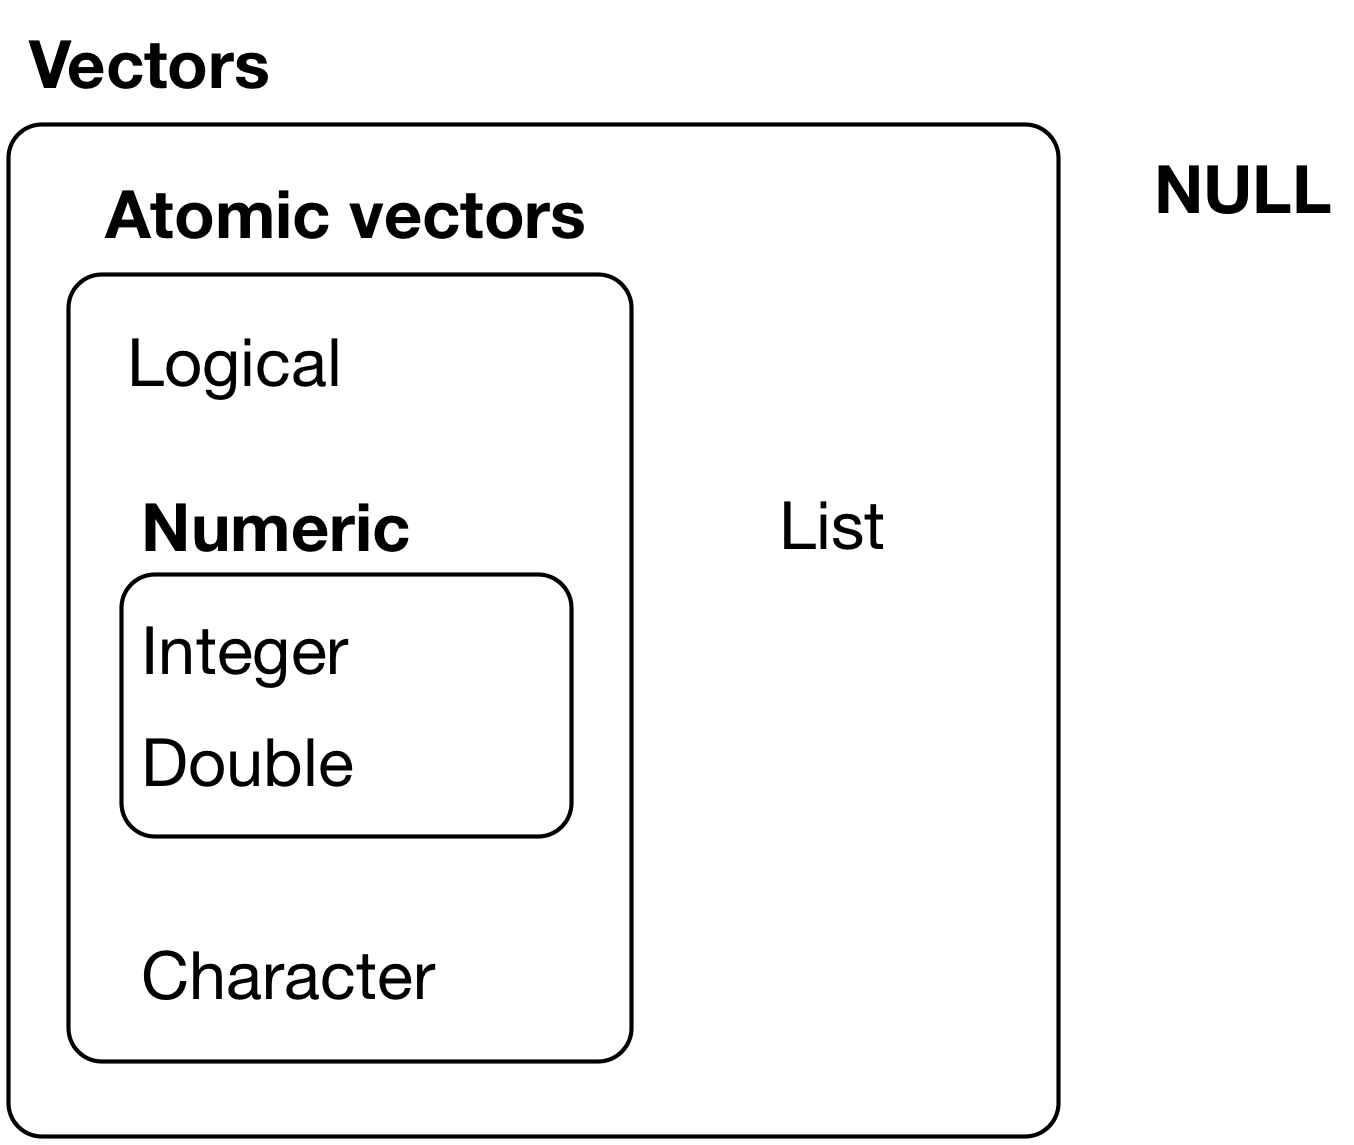
\includegraphics{../img/data-structures-overview.png}
\caption{Hierarchy of R's vector types}
\end{figure}

\end{frame}

\begin{frame}[fragile]{ベクトルのプロパティ}

\begin{block}{型}

\begin{Shaded}
\begin{Highlighting}[]
\KeywordTok{typeof}\NormalTok{(}\DecValTok{1}\OperatorTok{:}\DecValTok{10}\NormalTok{)}
\end{Highlighting}
\end{Shaded}

\begin{verbatim}
## [1] "integer"
\end{verbatim}

\begin{Shaded}
\begin{Highlighting}[]
\KeywordTok{typeof}\NormalTok{(}\KeywordTok{list}\NormalTok{(}\DecValTok{1}\NormalTok{,}\StringTok{"a"}\NormalTok{))}
\end{Highlighting}
\end{Shaded}

\begin{verbatim}
## [1] "list"
\end{verbatim}

\end{block}

\begin{block}{長さ}

\begin{Shaded}
\begin{Highlighting}[]
\KeywordTok{length}\NormalTok{(}\DecValTok{1}\OperatorTok{:}\DecValTok{10}\NormalTok{)}
\end{Highlighting}
\end{Shaded}

\begin{verbatim}
## [1] 10
\end{verbatim}

\end{block}

\end{frame}

\begin{frame}{拡張されたベクトル}

一部のベクトルは\textbf{属性(attribute)}という付加情報を持たせて複雑な操作ができる。

\begin{itemize}
\tightlist
\item
  factor:実体はintegerベクトル
\item
  date: 実体はdoubleベクトル
\item
  data.frame: 実体はリスト
\end{itemize}

\end{frame}

\begin{frame}{20.3 Important types of atomic vector}

\begin{itemize}
\tightlist
\item
  logical, integer, double, character

  \begin{itemize}
  \tightlist
  \item
    complex, rawは扱わない
  \end{itemize}
\end{itemize}

\end{frame}

\begin{frame}[fragile]{20.3.1 Logical}

最も原子的

\begin{block}{値}

\texttt{TRUE}, \texttt{FALSE}, \texttt{NA}の三種類のみ

\end{block}

\begin{block}{生成}

\begin{Shaded}
\begin{Highlighting}[]
\DecValTok{1}\OperatorTok{:}\DecValTok{10} \OperatorTok\StringTok{ }\DecValTok{3} \OperatorTok{==}\StringTok{ }\DecValTok{0}
\end{Highlighting}
\end{Shaded}

\begin{verbatim}
##  [1] FALSE FALSE  TRUE FALSE FALSE  TRUE FALSE FALSE  TRUE FALSE
\end{verbatim}

\begin{Shaded}
\begin{Highlighting}[]
\KeywordTok{c}\NormalTok{(}\OtherTok{TRUE}\NormalTok{, }\OtherTok{TRUE}\NormalTok{, }\OtherTok{FALSE}\NormalTok{, }\OtherTok{NA}\NormalTok{)}
\end{Highlighting}
\end{Shaded}

\begin{verbatim}
## [1]  TRUE  TRUE FALSE    NA
\end{verbatim}

\end{block}

\end{frame}

\begin{frame}[fragile]{20.3.2 Numeric}

Logicalの次に原子的

二種類に分類できる - integer - double(デフォルト)

\begin{Shaded}
\begin{Highlighting}[]
\KeywordTok{typeof}\NormalTok{(}\DecValTok{1}\NormalTok{)}
\end{Highlighting}
\end{Shaded}

\begin{verbatim}
## [1] "double"
\end{verbatim}

\begin{Shaded}
\begin{Highlighting}[]
\KeywordTok{typeof}\NormalTok{(1L)}
\end{Highlighting}
\end{Shaded}

\begin{verbatim}
## [1] "integer"
\end{verbatim}

\end{frame}

\begin{frame}[fragile]{doubleは近似}

\begin{Shaded}
\begin{Highlighting}[]
\NormalTok{x <-}\StringTok{ }\KeywordTok{sqrt}\NormalTok{(}\DecValTok{2}\NormalTok{) }\OperatorTok{^}\StringTok{ }\DecValTok{2}
\NormalTok{x}
\end{Highlighting}
\end{Shaded}

\begin{verbatim}
## [1] 2
\end{verbatim}

\begin{Shaded}
\begin{Highlighting}[]
\NormalTok{x }\OperatorTok{-}\StringTok{ }\DecValTok{2}
\end{Highlighting}
\end{Shaded}

\begin{verbatim}
## [1] 4.440892e-16
\end{verbatim}

\begin{block}{教訓}

\texttt{==}じゃなくて\texttt{near}を使う

\end{block}

\end{frame}

\begin{frame}[fragile]{特殊な値}

\begin{itemize}
\tightlist
\item
  \texttt{NA}
\item
  \texttt{NaN} (doubleのみ)
\item
  \texttt{Inf}, \texttt{-Inf} (doubleのみ)
\end{itemize}

\begin{block}{check}

\texttt{is.na}, \texttt{is.finite}, \texttt{is.nan}

\end{block}

\end{frame}

\begin{frame}{20.3.3 Character}

要素は任意の文字列

データの大きさが一定でない

\end{frame}

\begin{frame}[fragile]{Global string pool}

文字列の実体は一箇所に保管されている

\(\Rightarrow\) データの実体はpoolへのリンク

\begin{Shaded}
\begin{Highlighting}[]
\NormalTok{x <-}\StringTok{ "This is a reasonably long string."}
\NormalTok{pryr}\OperatorTok{::}\KeywordTok{object_size}\NormalTok{(x)}
\end{Highlighting}
\end{Shaded}

\begin{verbatim}
## 152 B
\end{verbatim}

\begin{Shaded}
\begin{Highlighting}[]
\NormalTok{y <-}\StringTok{ }\KeywordTok{rep}\NormalTok{(x, }\DecValTok{1000}\NormalTok{)}
\NormalTok{pryr}\OperatorTok{::}\KeywordTok{object_size}\NormalTok{(y)}
\end{Highlighting}
\end{Shaded}

\begin{verbatim}
## 8.14 kB
\end{verbatim}

\end{frame}

\begin{frame}[fragile]{20.3.4 Missing values}

実は\texttt{NA}にも型が存在する

\begin{Shaded}
\begin{Highlighting}[]
\OtherTok{NA}            \CommentTok{# logical}
\OtherTok{NA_integer_}   \CommentTok{# integer}
\OtherTok{NA_real_}      \CommentTok{# double}
\OtherTok{NA_character_} \CommentTok{# character}
\end{Highlighting}
\end{Shaded}

\end{frame}

\begin{frame}{20.3.5 Exercises}

\end{frame}

\begin{frame}{20.4 Using atomic vectors}

\begin{enumerate}
\def\labelenumi{\arabic{enumi}.}
\tightlist
\item
  どうやって型を変換するか
\item
  ベクトルの型の調べ方
\item
  異なる長さのベクトルがどのように作用するか
\item
  ベクトルの要素に名前を付ける方法
\item
  ベクトルの要素の抽出方法
\end{enumerate}

\end{frame}

\begin{frame}{20.4.1 Coercion}

型の変換

明示的(Explicit)な方法と暗黙的(Implicit)な方法

\end{frame}

\begin{frame}[fragile]{明示的な方法}

関数

\begin{itemize}
\tightlist
\item
  \texttt{as.logical}
\item
  \texttt{as.integer}
\item
  \texttt{as.double}
\item
  \texttt{as.character}
\end{itemize}

logical \textgreater{} integer \textgreater{} double \textgreater{}
character

の順に変換すればとりあえず間違いない。

逆も不可能ではないけど扱いに注意

\end{frame}

\begin{frame}[fragile]{暗黙的な方法: 例1}

logicalを実数として処理する方法

\begin{Shaded}
\begin{Highlighting}[]
\NormalTok{x <-}\StringTok{ }\KeywordTok{sample}\NormalTok{(}\DecValTok{20}\NormalTok{, }\DecValTok{100}\NormalTok{, }\DataTypeTok{replace =} \OtherTok{TRUE}\NormalTok{)}
\KeywordTok{sum}\NormalTok{(x }\OperatorTok{>}\StringTok{ }\DecValTok{10}\NormalTok{)  }\CommentTok{# how many are greater than 10?}
\end{Highlighting}
\end{Shaded}

\begin{verbatim}
## [1] 61
\end{verbatim}

\texttt{TRUE}は\texttt{1}に、\texttt{FALSE}は\texttt{0}になる

\end{frame}

\begin{frame}[fragile]{暗黙的な方法: 例2}

異なる型の値(ベクトル)を\texttt{c}で結合

\begin{Shaded}
\begin{Highlighting}[]
\KeywordTok{typeof}\NormalTok{(}\KeywordTok{c}\NormalTok{(}\OtherTok{TRUE}\NormalTok{, 1L))}
\end{Highlighting}
\end{Shaded}

\begin{verbatim}
## [1] "integer"
\end{verbatim}

\begin{Shaded}
\begin{Highlighting}[]
\KeywordTok{typeof}\NormalTok{(}\KeywordTok{c}\NormalTok{(}\FloatTok{1.5}\NormalTok{, }\StringTok{"a"}\NormalTok{))}
\end{Highlighting}
\end{Shaded}

\begin{verbatim}
## [1] "character"
\end{verbatim}

logical \textgreater{} integer \textgreater{} double \textgreater{}
complex \textgreater{} character\\
の強さの順で統一される

\begin{block}{はっきりと認識しておくこと}

ベクトルは複数種類の型の値を要素に持つことはできない

\end{block}

\end{frame}

\begin{frame}[fragile]{20.4.2 Test functions}

どの型のアトミックなのかテストする関数

\begin{longtable}[]{@{}llllll@{}}
\toprule
& lgl & int & dbl & chr & list\tabularnewline
\midrule
\endhead
\texttt{is\_logical} & x & & & &\tabularnewline
\texttt{is\_integer} & & x & & &\tabularnewline
\texttt{is\_double} & & & x & &\tabularnewline
\texttt{is\_numeric} & & x & x & &\tabularnewline
\texttt{is\_character} & & & & x &\tabularnewline
\texttt{is\_atomic} & x & x & x & x &\tabularnewline
\texttt{is\_list} & & & & & x\tabularnewline
\texttt{is\_vector} & x & x & x & x & x\tabularnewline
\bottomrule
\end{longtable}

\begin{block}{scalar}

\texttt{is\_scalar\_logical}で長さ1のlglかどうかテスト

\end{block}

\end{frame}

\begin{frame}{20.4.3 Scalars and recycling rules}

アトミックベクトルどおしの演算

\end{frame}

\begin{frame}[fragile]{基本ルール}

要素ごとに演算される

\begin{Shaded}
\begin{Highlighting}[]
\KeywordTok{c}\NormalTok{(}\DecValTok{1}\NormalTok{, }\DecValTok{2}\NormalTok{, }\DecValTok{3}\NormalTok{) }\OperatorTok{*}\StringTok{ }\KeywordTok{c}\NormalTok{(}\DecValTok{1}\NormalTok{, }\DecValTok{10}\NormalTok{, }\DecValTok{100}\NormalTok{)}
\end{Highlighting}
\end{Shaded}

\begin{verbatim}
## [1]   1  20 300
\end{verbatim}

長さが違う場合は?

\end{frame}

\begin{frame}[fragile]{リサイクル}

演算入力のベクトルの長さが異なる場合は短い方が繰り返される

\begin{Shaded}
\begin{Highlighting}[]
\DecValTok{1}\OperatorTok{:}\DecValTok{10} \OperatorTok{+}\StringTok{ }\DecValTok{100}
\end{Highlighting}
\end{Shaded}

\begin{verbatim}
##  [1] 101 102 103 104 105 106 107 108 109 110
\end{verbatim}

\begin{Shaded}
\begin{Highlighting}[]
\DecValTok{1}\OperatorTok{:}\DecValTok{10} \OperatorTok{+}\StringTok{ }\DecValTok{1}\OperatorTok{:}\DecValTok{2} \OperatorTok{*}\StringTok{ }\DecValTok{100}
\end{Highlighting}
\end{Shaded}

\begin{verbatim}
##  [1] 101 202 103 204 105 206 107 208 109 210
\end{verbatim}

\end{frame}

\begin{frame}[fragile]{リサイクル2}

繰り返し回数が合わなければ途中までリサイクル

\begin{Shaded}
\begin{Highlighting}[]
\DecValTok{1}\OperatorTok{:}\DecValTok{10} \OperatorTok{+}\StringTok{ }\DecValTok{1}\OperatorTok{:}\DecValTok{3} \OperatorTok{*}\StringTok{ }\DecValTok{100}
\end{Highlighting}
\end{Shaded}

\begin{verbatim}
## Warning in 1:10 + 1:3 * 100: longer object length is not a multiple of
## shorter object length
\end{verbatim}

\begin{verbatim}
##  [1] 101 202 303 104 205 306 107 208 309 110
\end{verbatim}

\end{frame}

\begin{frame}[fragile]{\texttt{tidyverse}}

\texttt{tidyverse}な世界ではベクトル-スカラー以外のリサイクルは禁止

\begin{Shaded}
\begin{Highlighting}[]
\KeywordTok{tibble}\NormalTok{(}\DataTypeTok{x =} \DecValTok{1}\OperatorTok{:}\DecValTok{3}\NormalTok{, }\DataTypeTok{y =} \DecValTok{1}\NormalTok{)}
\end{Highlighting}
\end{Shaded}

\begin{verbatim}
## # A tibble: 3 x 2
##       x     y
##   <int> <dbl>
## 1     1     1
## 2     2     1
## 3     3     1
\end{verbatim}

\begin{Shaded}
\begin{Highlighting}[]
\KeywordTok{tibble}\NormalTok{(}\DataTypeTok{x =} \DecValTok{1}\OperatorTok{:}\DecValTok{3}\NormalTok{, }\DataTypeTok{y =} \DecValTok{1}\OperatorTok{:}\DecValTok{2}\NormalTok{)}
\end{Highlighting}
\end{Shaded}

\begin{verbatim}
## Tibble columns must have consistent lengths, only values of length one are recycled:
## * Length 2: Column `y`
## * Length 3: Column `x`
\end{verbatim}

\end{frame}

\begin{frame}{20.4.4 Naming vectors}

ベクトル要素に名前をつける

\end{frame}

\begin{frame}[fragile]{ベクトル要素の名前}

\begin{Shaded}
\begin{Highlighting}[]
\NormalTok{v <-}\StringTok{ }\KeywordTok{c}\NormalTok{(}\DataTypeTok{x =} \DecValTok{1}\NormalTok{, }\DataTypeTok{y =} \DecValTok{2}\NormalTok{, }\DataTypeTok{z =} \DecValTok{4}\NormalTok{)}
\NormalTok{v}
\end{Highlighting}
\end{Shaded}

\begin{verbatim}
## x y z 
## 1 2 4
\end{verbatim}

\begin{Shaded}
\begin{Highlighting}[]
\KeywordTok{names}\NormalTok{(v)}
\end{Highlighting}
\end{Shaded}

\begin{verbatim}
## [1] "x" "y" "z"
\end{verbatim}

\end{frame}

\begin{frame}[fragile]{名前の変更}

\begin{Shaded}
\begin{Highlighting}[]
\NormalTok{v }\OperatorTok\StringTok{ }\KeywordTok{set_names}\NormalTok{(}\KeywordTok{c}\NormalTok{(}\StringTok{"a"}\NormalTok{, }\StringTok{"b"}\NormalTok{, }\StringTok{"c"}\NormalTok{))}
\end{Highlighting}
\end{Shaded}

\begin{verbatim}
## a b c 
## 1 2 4
\end{verbatim}

\end{frame}

\begin{frame}[fragile]{20.4.5 Subsetting}

ベクトルの一部の要素を抽出する

\begin{block}{operator}

ベクトルの後ろに\texttt{{[}...{]}}を付ける

\texttt{{[}...{]}}の中に入れる値は三種類

\begin{itemize}
\tightlist
\item
  index
\item
  logical
\item
  name strings
\end{itemize}

\end{block}

\end{frame}

\begin{frame}[fragile]{index}

前から数えた位置で指定する

\begin{Shaded}
\begin{Highlighting}[]
\NormalTok{x <-}\StringTok{ }\KeywordTok{c}\NormalTok{(}\StringTok{"one"}\NormalTok{, }\StringTok{"two"}\NormalTok{, }\StringTok{"three"}\NormalTok{, }\StringTok{"four"}\NormalTok{, }\StringTok{"five"}\NormalTok{)}
\NormalTok{x[}\KeywordTok{c}\NormalTok{(}\DecValTok{3}\NormalTok{, }\DecValTok{2}\NormalTok{, }\DecValTok{5}\NormalTok{)] }
\end{Highlighting}
\end{Shaded}

\begin{verbatim}
## [1] "three" "two"   "five"
\end{verbatim}

\begin{Shaded}
\begin{Highlighting}[]
\NormalTok{x[}\KeywordTok{c}\NormalTok{(}\DecValTok{1}\NormalTok{, }\DecValTok{1}\NormalTok{, }\DecValTok{5}\NormalTok{, }\DecValTok{5}\NormalTok{, }\DecValTok{5}\NormalTok{, }\DecValTok{2}\NormalTok{)] }\CommentTok{#繰り返し}
\end{Highlighting}
\end{Shaded}

\begin{verbatim}
## [1] "one"  "one"  "five" "five" "five" "two"
\end{verbatim}

\begin{Shaded}
\begin{Highlighting}[]
\NormalTok{x[}\KeywordTok{c}\NormalTok{(}\OperatorTok{-}\DecValTok{1}\NormalTok{, }\OperatorTok{-}\DecValTok{3}\NormalTok{, }\OperatorTok{-}\DecValTok{5}\NormalTok{)] }\CommentTok{#マイナス指定}
\end{Highlighting}
\end{Shaded}

\begin{verbatim}
## [1] "two"  "four"
\end{verbatim}

\end{frame}

\begin{frame}[fragile]{logical}

元と同じ長さの論理ベクトルの\texttt{TRUE}の位置で指定

\begin{Shaded}
\begin{Highlighting}[]
\NormalTok{x <-}\StringTok{ }\KeywordTok{c}\NormalTok{(}\DecValTok{10}\NormalTok{, }\DecValTok{3}\NormalTok{, }\OtherTok{NA}\NormalTok{, }\DecValTok{5}\NormalTok{, }\DecValTok{8}\NormalTok{, }\DecValTok{1}\NormalTok{, }\OtherTok{NA}\NormalTok{)}
\NormalTok{x[}\OperatorTok{!}\KeywordTok{is.na}\NormalTok{(x)] }\CommentTok{#NAを除く}
\end{Highlighting}
\end{Shaded}

\begin{verbatim}
## [1] 10  3  5  8  1
\end{verbatim}

\begin{Shaded}
\begin{Highlighting}[]
\NormalTok{x[x }\OperatorTok\StringTok{ }\DecValTok{2} \OperatorTok{==}\StringTok{ }\DecValTok{0}\NormalTok{] }\CommentTok{#偶数とNA}
\end{Highlighting}
\end{Shaded}

\begin{verbatim}
## [1] 10 NA  8 NA
\end{verbatim}

\end{frame}

\begin{frame}[fragile]{name strings}

ベクトル要素の名前で指定

\begin{Shaded}
\begin{Highlighting}[]
\NormalTok{x <-}\StringTok{ }\KeywordTok{c}\NormalTok{(}\DataTypeTok{abc =} \DecValTok{1}\NormalTok{, }\DataTypeTok{def =} \DecValTok{2}\NormalTok{, }\DataTypeTok{xyz =} \DecValTok{5}\NormalTok{)}
\NormalTok{x[}\KeywordTok{c}\NormalTok{(}\StringTok{"xyz"}\NormalTok{, }\StringTok{"def"}\NormalTok{)]}
\end{Highlighting}
\end{Shaded}

\begin{verbatim}
## xyz def 
##   5   2
\end{verbatim}

\end{frame}

\begin{frame}[fragile]{nothing}

要素を指定せずに全体を得る

\begin{Shaded}
\begin{Highlighting}[]
\NormalTok{iris[}\DecValTok{1}\NormalTok{,]}
\end{Highlighting}
\end{Shaded}

\begin{verbatim}
##   Sepal.Length Sepal.Width Petal.Length Petal.Width Species
## 1          5.1         3.5          1.4         0.2  setosa
\end{verbatim}

\begin{Shaded}
\begin{Highlighting}[]
\NormalTok{iris[,}\DecValTok{1}\NormalTok{]}
\end{Highlighting}
\end{Shaded}

\begin{verbatim}
##   [1] 5.1 4.9 4.7 4.6 5.0 5.4 4.6 5.0 4.4 4.9 5.4 4.8 4.8 4.3 5.8 5.7 5.4
##  [18] 5.1 5.7 5.1 5.4 5.1 4.6 5.1 4.8 5.0 5.0 5.2 5.2 4.7 4.8 5.4 5.2 5.5
##  [35] 4.9 5.0 5.5 4.9 4.4 5.1 5.0 4.5 4.4 5.0 5.1 4.8 5.1 4.6 5.3 5.0 7.0
##  [52] 6.4 6.9 5.5 6.5 5.7 6.3 4.9 6.6 5.2 5.0 5.9 6.0 6.1 5.6 6.7 5.6 5.8
##  [69] 6.2 5.6 5.9 6.1 6.3 6.1 6.4 6.6 6.8 6.7 6.0 5.7 5.5 5.5 5.8 6.0 5.4
##  [86] 6.0 6.7 6.3 5.6 5.5 5.5 6.1 5.8 5.0 5.6 5.7 5.7 6.2 5.1 5.7 6.3 5.8
## [103] 7.1 6.3 6.5 7.6 4.9 7.3 6.7 7.2 6.5 6.4 6.8 5.7 5.8 6.4 6.5 7.7 7.7
## [120] 6.0 6.9 5.6 7.7 6.3 6.7 7.2 6.2 6.1 6.4 7.2 7.4 7.9 6.4 6.3 6.1 7.7
## [137] 6.3 6.4 6.0 6.9 6.7 6.9 5.8 6.8 6.7 6.7 6.3 6.5 6.2 5.9
\end{verbatim}

\end{frame}

\begin{frame}[fragile]{subsetting function}

実は関数\texttt{"{[}"}がコールされている

\begin{Shaded}
\begin{Highlighting}[]
\StringTok{"["}\NormalTok{(x, }\DecValTok{1}\NormalTok{)}
\end{Highlighting}
\end{Shaded}

\begin{verbatim}
## abc 
##   1
\end{verbatim}

\begin{Shaded}
\begin{Highlighting}[]
\NormalTok{x }\OperatorTok\StringTok{ "["}\NormalTok{(}\DecValTok{1}\NormalTok{)}
\end{Highlighting}
\end{Shaded}

\begin{verbatim}
## abc 
##   1
\end{verbatim}

\end{frame}

\begin{frame}{20.4.6 Exercises}

\end{frame}

\begin{frame}{20.5 Recursive vectors (lists)}

制約が無さ過ぎるベクトル

\end{frame}

\begin{frame}[fragile]{型の制約なし}

アトミックのように要素の型が統一されている必要がない

\begin{Shaded}
\begin{Highlighting}[]
\NormalTok{y <-}\StringTok{ }\KeywordTok{list}\NormalTok{(}\StringTok{"a"}\NormalTok{, 1L, }\FloatTok{1.5}\NormalTok{, }\OtherTok{TRUE}\NormalTok{)}
\KeywordTok{str}\NormalTok{(y)}
\end{Highlighting}
\end{Shaded}

\begin{verbatim}
## List of 4
##  $ : chr "a"
##  $ : int 1
##  $ : num 1.5
##  $ : logi TRUE
\end{verbatim}

\end{frame}

\begin{frame}[fragile]{繰り返し}

listはlistを要素に持てる

\begin{Shaded}
\begin{Highlighting}[]
\NormalTok{z <-}\StringTok{ }\KeywordTok{list}\NormalTok{(}\KeywordTok{list}\NormalTok{(}\DecValTok{1}\NormalTok{, }\DecValTok{2}\NormalTok{), }\KeywordTok{list}\NormalTok{(}\DecValTok{3}\NormalTok{, }\DecValTok{4}\NormalTok{, }\DecValTok{5}\NormalTok{))}
\KeywordTok{str}\NormalTok{(z)}
\end{Highlighting}
\end{Shaded}

\begin{verbatim}
## List of 2
##  $ :List of 2
##   ..$ : num 1
##   ..$ : num 2
##  $ :List of 3
##   ..$ : num 3
##   ..$ : num 4
##   ..$ : num 5
\end{verbatim}

\end{frame}

\begin{frame}{20.5.1 Visualising lists}

list構造の可視化方法

この本のためのHadleyさんオリジナル

\end{frame}

\begin{frame}[fragile]{リストの可視化ルール}

\begin{Shaded}
\begin{Highlighting}[]
\NormalTok{x1 <-}\StringTok{ }\KeywordTok{list}\NormalTok{(}\KeywordTok{c}\NormalTok{(}\DecValTok{1}\NormalTok{, }\DecValTok{2}\NormalTok{), }\KeywordTok{c}\NormalTok{(}\DecValTok{3}\NormalTok{, }\DecValTok{4}\NormalTok{))}
\NormalTok{x2 <-}\StringTok{ }\KeywordTok{list}\NormalTok{(}\KeywordTok{list}\NormalTok{(}\DecValTok{1}\NormalTok{, }\DecValTok{2}\NormalTok{), }\KeywordTok{list}\NormalTok{(}\DecValTok{3}\NormalTok{, }\DecValTok{4}\NormalTok{))}
\NormalTok{x3 <-}\StringTok{ }\KeywordTok{list}\NormalTok{(}\DecValTok{1}\NormalTok{, }\KeywordTok{list}\NormalTok{(}\DecValTok{2}\NormalTok{, }\KeywordTok{list}\NormalTok{(}\DecValTok{3}\NormalTok{)))}
\end{Highlighting}
\end{Shaded}

\begin{center}
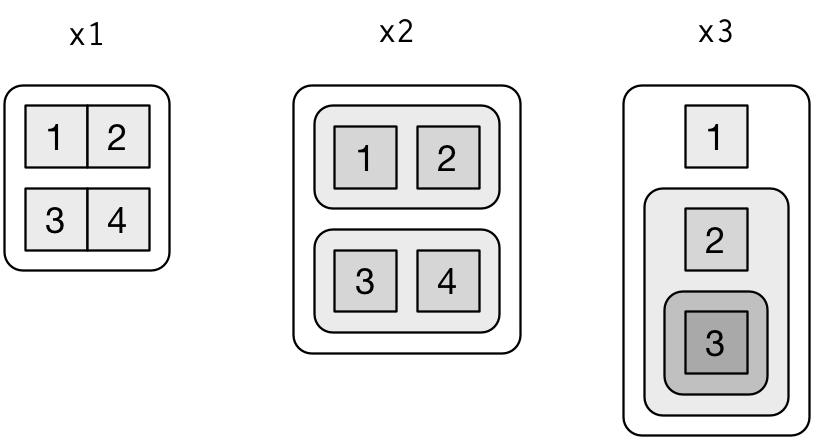
\includegraphics[width=80mm]{../img/lists-structure.png}
\end{center}

\begin{itemize}
\tightlist
\item
  リストは角が丸、アトミックは四角
\item
  子は親の中に入れる。階層が深いとグレー
\item
  向きや順序に意味はない
\end{itemize}

\end{frame}

\begin{frame}[fragile]{20.5.2 Subsetting}

リストには三種の要素抽出方法がある

\begin{Shaded}
\begin{Highlighting}[]
\NormalTok{a <-}\StringTok{ }\KeywordTok{list}\NormalTok{(}\DataTypeTok{a =} \DecValTok{1}\OperatorTok{:}\DecValTok{3}\NormalTok{, }\DataTypeTok{b =} \StringTok{"a string"}\NormalTok{, }\DataTypeTok{c =}\NormalTok{ pi, }\DataTypeTok{d =} \KeywordTok{list}\NormalTok{(}\OperatorTok{-}\DecValTok{1}\NormalTok{, }\OperatorTok{-}\DecValTok{5}\NormalTok{))}
\NormalTok{a[}\DecValTok{1}\NormalTok{]}
\end{Highlighting}
\end{Shaded}

\begin{verbatim}
## $a
## [1] 1 2 3
\end{verbatim}

\begin{Shaded}
\begin{Highlighting}[]
\NormalTok{a[[}\DecValTok{1}\NormalTok{]]}
\end{Highlighting}
\end{Shaded}

\begin{verbatim}
## [1] 1 2 3
\end{verbatim}

\begin{Shaded}
\begin{Highlighting}[]
\NormalTok{a}\OperatorTok{$}\NormalTok{a}
\end{Highlighting}
\end{Shaded}

\begin{verbatim}
## [1] 1 2 3
\end{verbatim}

\end{frame}

\begin{frame}{可視化}

\begin{figure}
\centering
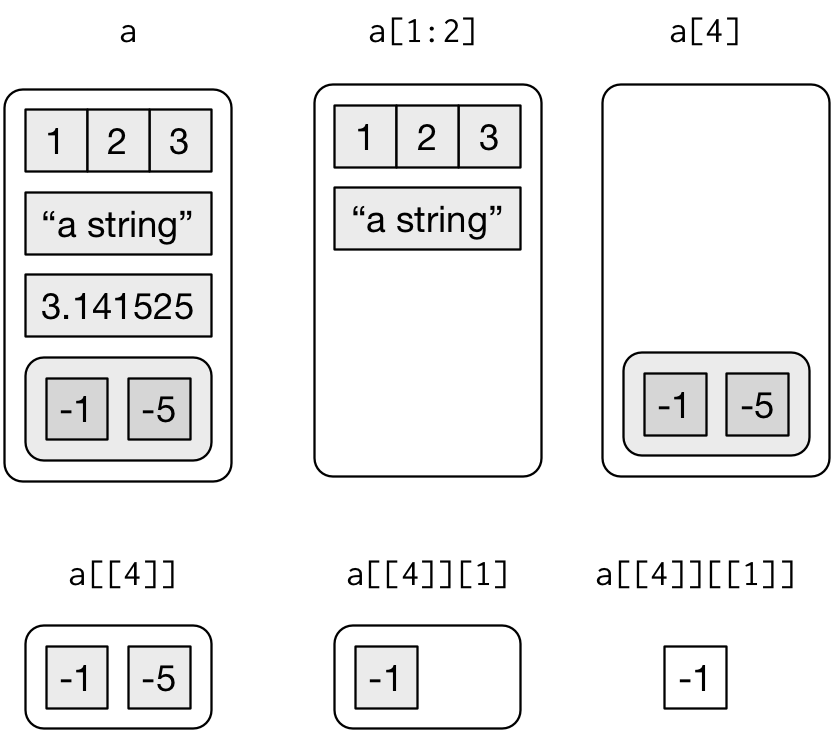
\includegraphics[width=0.80000\textwidth]{../img/lists-subsetting.png}
\caption{Subsetting a list, visually}
\end{figure}

\end{frame}

\begin{frame}[fragile]{20.5.3 Lists of condiments}

たとえ話

\begin{longtable}[]{@{}cccc@{}}
\toprule
\texttt{a} & \texttt{a{[}1{]}} & \texttt{a{[}{[}1{]}{]}} &
\texttt{a{[}{[}1{]}{]}{[}{[}1{]}{]}}\tabularnewline
\midrule
\endhead

\includegraphics[width=0.20000\textwidth]{../img/pepper.jpg} &
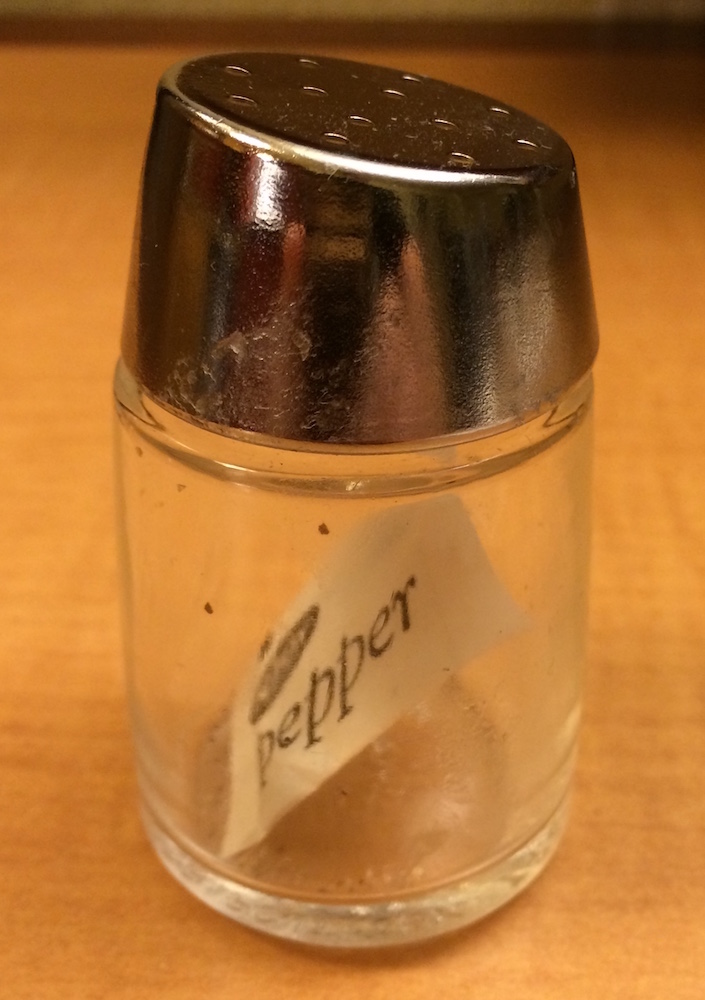
\includegraphics[width=0.20000\textwidth]{../img/pepper-1.jpg} &
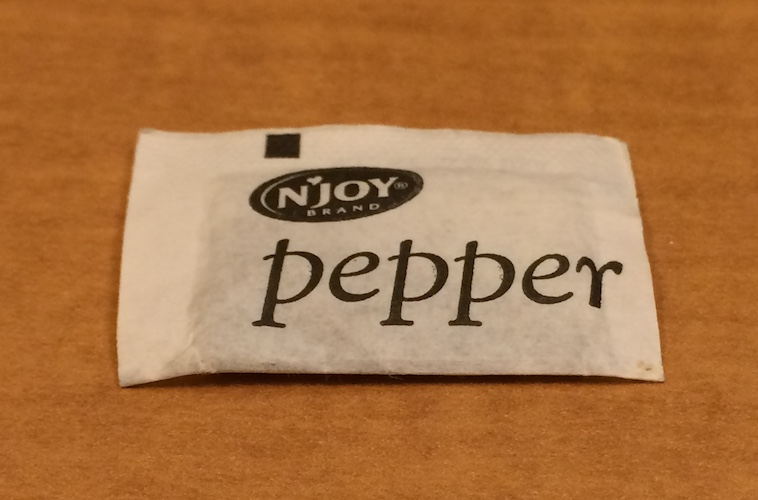
\includegraphics[width=0.20000\textwidth]{../img/pepper-2.jpg} &
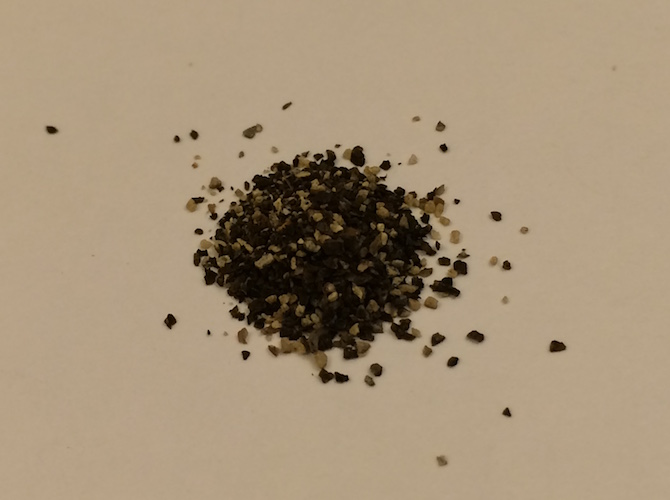
\includegraphics[width=0.20000\textwidth]{../img/pepper-3.jpg}\tabularnewline
\bottomrule
\end{longtable}

\end{frame}

\begin{frame}{20.5.4 Exercises}

\end{frame}

\begin{frame}{20.6 Attributes}

ベクトルの属性(付加的な情報)

\end{frame}

\begin{frame}[fragile]{設定方法}

\begin{Shaded}
\begin{Highlighting}[]
\NormalTok{x <-}\StringTok{ }\DecValTok{1}\OperatorTok{:}\DecValTok{10}
\KeywordTok{attr}\NormalTok{(x, }\StringTok{"greeting"}\NormalTok{)}
\end{Highlighting}
\end{Shaded}

\begin{verbatim}
## NULL
\end{verbatim}

\begin{Shaded}
\begin{Highlighting}[]
\KeywordTok{attr}\NormalTok{(x, }\StringTok{"greeting"}\NormalTok{) <-}\StringTok{ "Hi!"}
\KeywordTok{attr}\NormalTok{(x, }\StringTok{"farewell"}\NormalTok{) <-}\StringTok{ "Bye!"}
\KeywordTok{attributes}\NormalTok{(x)}
\end{Highlighting}
\end{Shaded}

\begin{verbatim}
## $greeting
## [1] "Hi!"
## 
## $farewell
## [1] "Bye!"
\end{verbatim}

\end{frame}

\begin{frame}{重要な属性}

\begin{enumerate}
\def\labelenumi{\arabic{enumi}.}
\tightlist
\item
  names: 要素の名前
\item
  dimensions: 横や縦の次元を与えればベクトルを行列にできる
\item
  class: S3オブジェクト指向プログラミングのために使う

  \begin{itemize}
  \tightlist
  \item
    汎用関数の作用を制御する
  \end{itemize}
\end{enumerate}

\end{frame}

\begin{frame}[fragile]{汎用関数の例}

\begin{Shaded}
\begin{Highlighting}[]
\KeywordTok{as.Date}\NormalTok{(}\StringTok{"2019/8/20"}\NormalTok{)}
\end{Highlighting}
\end{Shaded}

\begin{verbatim}
## [1] "2019-08-20"
\end{verbatim}

\begin{Shaded}
\begin{Highlighting}[]
\KeywordTok{as.Date}\NormalTok{(}\DecValTok{18128}\NormalTok{)}
\end{Highlighting}
\end{Shaded}

\begin{verbatim}
## Error in as.Date.numeric(18128): 'origin' must be supplied
\end{verbatim}

\end{frame}

\begin{frame}[fragile]{もう一つの例}

\begin{Shaded}
\begin{Highlighting}[]
\KeywordTok{par}\NormalTok{(}\DataTypeTok{mfrow =} \KeywordTok{c}\NormalTok{(}\DecValTok{1}\NormalTok{,}\DecValTok{2}\NormalTok{))}
\KeywordTok{plot}\NormalTok{(cars)}
\KeywordTok{plot}\NormalTok{(}\KeywordTok{lm}\NormalTok{(dist }\OperatorTok{~}\StringTok{ }\NormalTok{speed, cars))}
\end{Highlighting}
\end{Shaded}

\includegraphics{ch20_vectors_files/figure-beamer/generic.plot-1.pdf}
\includegraphics{ch20_vectors_files/figure-beamer/generic.plot-2.pdf}
\includegraphics{ch20_vectors_files/figure-beamer/generic.plot-3.pdf}

\end{frame}

\begin{frame}{20.7 Augmented vectors}

attributesの実践的な活用例

\begin{itemize}
\tightlist
\item
  factor
\item
  dates
\item
  datetimes
\item
  tibbles
\end{itemize}

\end{frame}

\begin{frame}[fragile]{20.7.1 Factors}

\begin{Shaded}
\begin{Highlighting}[]
\NormalTok{x <-}\StringTok{ }\KeywordTok{factor}\NormalTok{(}\KeywordTok{c}\NormalTok{(}\StringTok{"ab"}\NormalTok{, }\StringTok{"cd"}\NormalTok{, }\StringTok{"ab"}\NormalTok{), }\DataTypeTok{levels =} \KeywordTok{c}\NormalTok{(}\StringTok{"ab"}\NormalTok{, }\StringTok{"cd"}\NormalTok{, }\StringTok{"ef"}\NormalTok{))}
\KeywordTok{typeof}\NormalTok{(x)}
\end{Highlighting}
\end{Shaded}

\begin{verbatim}
## [1] "integer"
\end{verbatim}

\begin{Shaded}
\begin{Highlighting}[]
\KeywordTok{attributes}\NormalTok{(x)}
\end{Highlighting}
\end{Shaded}

\begin{verbatim}
## $levels
## [1] "ab" "cd" "ef"
## 
## $class
## [1] "factor"
\end{verbatim}

\end{frame}

\begin{frame}[fragile]{20.7.2 Dates and datetimes}

\begin{block}{date}

\begin{Shaded}
\begin{Highlighting}[]
\NormalTok{x <-}\StringTok{ }\KeywordTok{as.Date}\NormalTok{(}\StringTok{"1971-01-01"}\NormalTok{)}
\KeywordTok{unclass}\NormalTok{(x)}
\end{Highlighting}
\end{Shaded}

\begin{verbatim}
## [1] 365
\end{verbatim}

\begin{Shaded}
\begin{Highlighting}[]
\KeywordTok{typeof}\NormalTok{(x)}
\end{Highlighting}
\end{Shaded}

\begin{verbatim}
## [1] "double"
\end{verbatim}

\begin{Shaded}
\begin{Highlighting}[]
\KeywordTok{attributes}\NormalTok{(x)}
\end{Highlighting}
\end{Shaded}

\begin{verbatim}
## $class
## [1] "Date"
\end{verbatim}

\end{block}

\end{frame}

\begin{frame}[fragile]{datetime}

\begin{Shaded}
\begin{Highlighting}[]
\NormalTok{x <-}\StringTok{ }\NormalTok{lubridate}\OperatorTok{::}\KeywordTok{ymd_hm}\NormalTok{(}\StringTok{"1970-01-01 01:00"}\NormalTok{)}
\KeywordTok{typeof}\NormalTok{(x)}
\end{Highlighting}
\end{Shaded}

\begin{verbatim}
## [1] "double"
\end{verbatim}

\begin{Shaded}
\begin{Highlighting}[]
\KeywordTok{attributes}\NormalTok{(x)}
\end{Highlighting}
\end{Shaded}

\begin{verbatim}
## $class
## [1] "POSIXct" "POSIXt" 
## 
## $tzone
## [1] "UTC"
\end{verbatim}

\end{frame}

\begin{frame}[fragile]{update attribute}

\begin{Shaded}
\begin{Highlighting}[]
\KeywordTok{attr}\NormalTok{(x, }\StringTok{"tzone"}\NormalTok{) <-}\StringTok{ "US/Pacific"}
\NormalTok{x}
\end{Highlighting}
\end{Shaded}

\begin{verbatim}
## [1] "1969-12-31 17:00:00 PST"
\end{verbatim}

\begin{Shaded}
\begin{Highlighting}[]
\KeywordTok{attr}\NormalTok{(x, }\StringTok{"tzone"}\NormalTok{) <-}\StringTok{ "US/Eastern"}
\NormalTok{x}
\end{Highlighting}
\end{Shaded}

\begin{verbatim}
## [1] "1969-12-31 20:00:00 EST"
\end{verbatim}

\end{frame}

\begin{frame}[fragile]{20.7.3 Tibbles}

\begin{Shaded}
\begin{Highlighting}[]
\NormalTok{tb <-}\StringTok{ }\NormalTok{tibble}\OperatorTok{::}\KeywordTok{tibble}\NormalTok{(}\DataTypeTok{x =} \DecValTok{1}\OperatorTok{:}\DecValTok{5}\NormalTok{, }\DataTypeTok{y =} \DecValTok{5}\OperatorTok{:}\DecValTok{1}\NormalTok{)}
\KeywordTok{typeof}\NormalTok{(tb)}
\end{Highlighting}
\end{Shaded}

\begin{verbatim}
## [1] "list"
\end{verbatim}

\begin{Shaded}
\begin{Highlighting}[]
\KeywordTok{attributes}\NormalTok{(tb)}
\end{Highlighting}
\end{Shaded}

\begin{verbatim}
## $names
## [1] "x" "y"
## 
## $row.names
## [1] 1 2 3 4 5
## 
## $class
## [1] "tbl_df"     "tbl"        "data.frame"
\end{verbatim}

\end{frame}

\begin{frame}[fragile]{dataframe}

\begin{Shaded}
\begin{Highlighting}[]
\NormalTok{df <-}\StringTok{ }\KeywordTok{data.frame}\NormalTok{(}\DataTypeTok{x =} \DecValTok{1}\OperatorTok{:}\DecValTok{5}\NormalTok{, }\DataTypeTok{y =} \DecValTok{5}\OperatorTok{:}\DecValTok{1}\NormalTok{)}
\KeywordTok{typeof}\NormalTok{(df)}
\end{Highlighting}
\end{Shaded}

\begin{verbatim}
## [1] "list"
\end{verbatim}

\begin{Shaded}
\begin{Highlighting}[]
\KeywordTok{attributes}\NormalTok{(df)}
\end{Highlighting}
\end{Shaded}

\begin{verbatim}
## $names
## [1] "x" "y"
## 
## $class
## [1] "data.frame"
## 
## $row.names
## [1] 1 2 3 4 5
\end{verbatim}

\end{frame}

\begin{frame}{20.7.4 Exercises}

\end{frame}

\begin{frame}{参考文献}

\begin{itemize}
\tightlist
\item
  \url{http://adv-r.had.co.nz/Functions.html\#lazy-evaluation}
\item
  \url{http://adv-r.had.co.nz/Subsetting.html\#applications}
\item
  \url{http://adv-r.had.co.nz/OO-essentials.html\#s3}
\end{itemize}

\end{frame}

\end{document}
